\documentclass{article}
\usepackage[T1]{fontenc}
\usepackage{lmodern}
\usepackage{graphicx}
\usepackage{amsmath,amssymb}
\usepackage[a4paper,margin=2cm]{geometry}
\usepackage[absolute,overlay]{textpos}
\setlength{\TPHorizModule}{1mm}
\setlength{\TPVertModule}{1mm}
\usepackage[indonesian]{babel}
\usepackage{hyperref}
\setlength{\emergencystretch}{2em}
% unit: Halaman 98

\begin{document}

% === Halaman 98 (llm) ===

\begin{itemize}
  \item Dekripsi perlu menghitung $\mathbf{K}^{-1}$ sedemikian sehingga $\mathbf{KK}^{-1} = \mathbf{I}$ ($\mathbf{I}$ matriks identitas).
\end{itemize}

\vspace{10mm}

sebaba

% deskripsi: Persamaan matriks untuk menentukan invers matriks K
% bbox normalisasi: [0.1200, 0.2500, 0.7800, 0.4300]
\begin{textblock*}{138.60mm}(25.20mm,74.25mm)
\noindent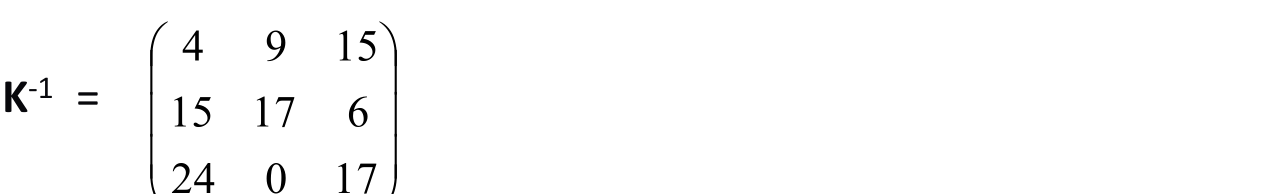
\includegraphics[width=138.60mm,height=53.46mm]{../../images/llm/page_098_img_01.png}%
\end{textblock*}

% deskripsi: Perhitungan perkalian matriks modulo 26 untuk membuktikan hasil invers
% bbox normalisasi: [0.1300, 0.5800, 0.7700, 0.7600]
\begin{textblock*}{134.40mm}(27.30mm,172.26mm)
\noindent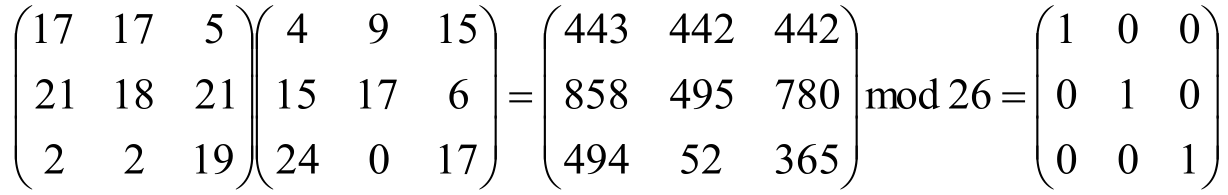
\includegraphics[width=134.40mm,height=53.46mm]{../../images/llm/page_098_img_02.png}%
\end{textblock*}

\end{document}
